
\chapter{Ugeopgave 5}
\label{cha:ugeopgave-5}

\section{Del 1}
\label{sec:del-1}

Hvis \emph{hidden surface}-algoritmen ikke er aktiveret, f�s
resultatet p� figur \ref{fig:5-1-1}. N�r \emph{hidden
  surface}-algoritmen aktiveres, fjernes kassen, som det kan ses p�
figur \ref{fig:5-1-2}.

\begin{figure}[hp]
\centering
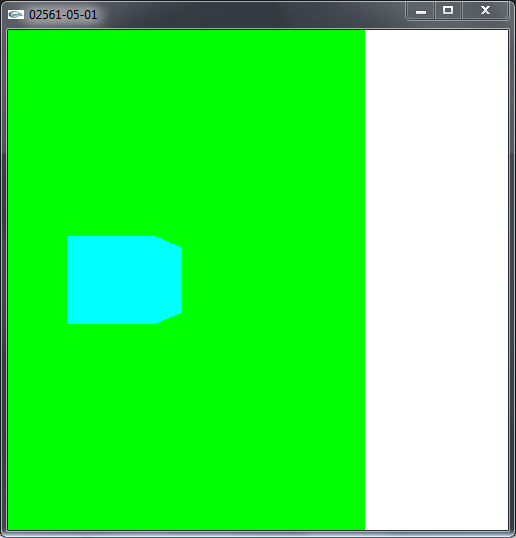
\includegraphics[width=8cm]{../exercise5/screenshots/part1_1.png}
\caption{Ingen \emph{hidden surface}}
\label{fig:5-1-1}
\end{figure}

\begin{figure}[hp]
\centering
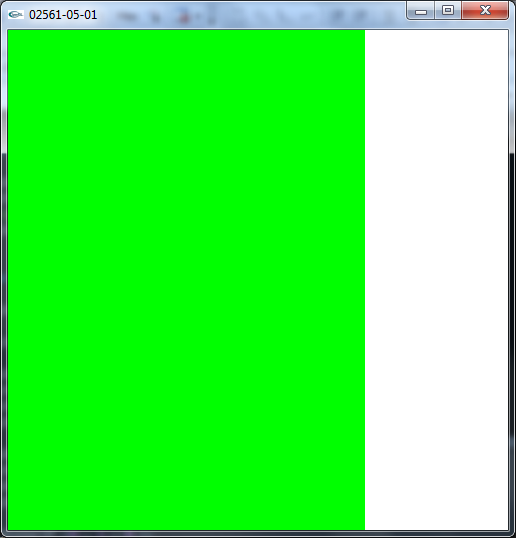
\includegraphics[width=8cm]{../exercise5/screenshots/part1_2.png}
\caption{Aktiveret \emph{hidden surface}}
\label{fig:5-1-2}
\end{figure}
